\documentclass{article}
\usepackage[margin=2.5cm]{geometry}
\usepackage{enumerate}
\usepackage{fancyhdr}
\usepackage{graphicx}
\usepackage{amsmath}

\pagestyle{fancy}
\fancyhead{}
\fancyfoot{}
\rfoot{\thepage}
\lfoot{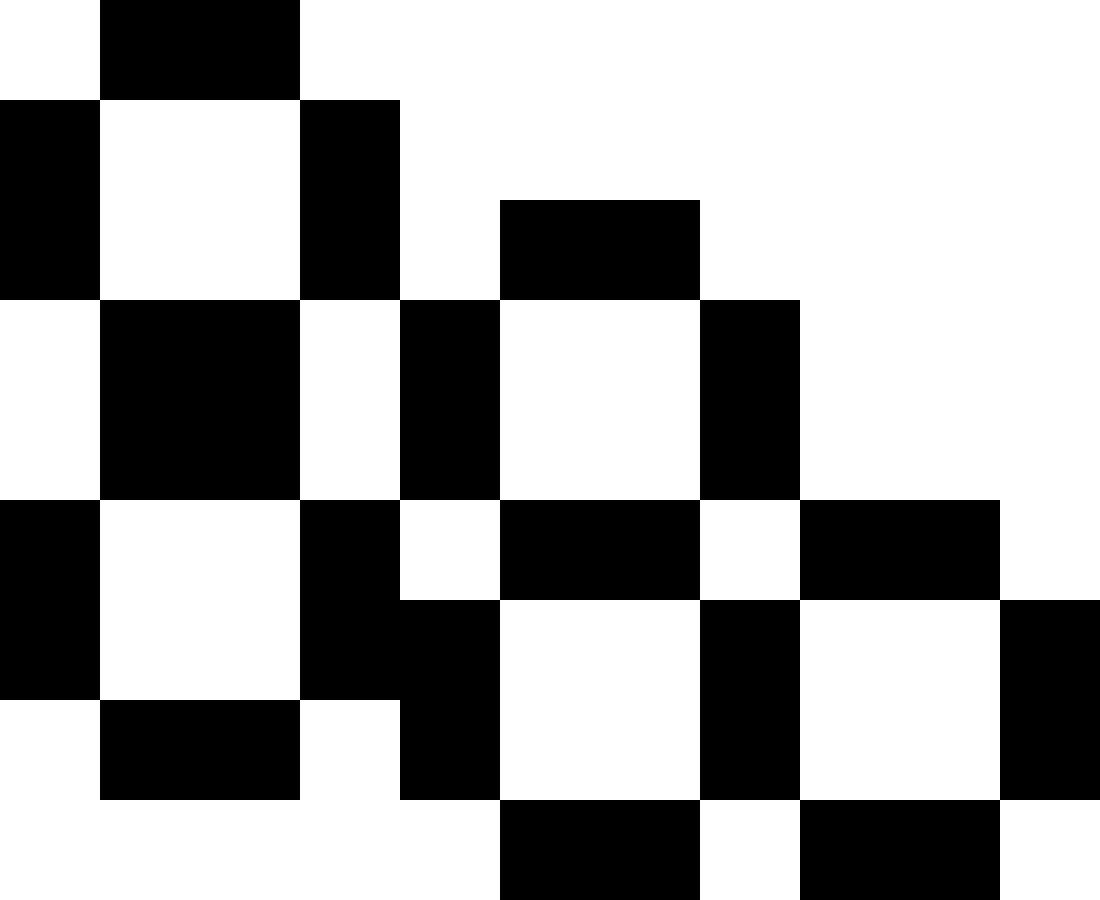
\includegraphics[height=20pt]{Logo}}

\usepackage{float}
\usepackage{listings, color, times, textcomp, float}
\definecolor{mygreen}{RGB}{28,172,0} % color values Red, Green, Blue
\definecolor{mylilas}{RGB}{170,55,241}
\lstset{language=Matlab, basicstyle=\scriptsize\ttfamily,breaklines=true,frame=single,morekeywords={matlab2tikz},
keywordstyle=\color{blue}, morekeywords=[2]{1}, keywordstyle=[2]{\color{black}}, identifierstyle=\color{black},
stringstyle=\color{mylilas}, commentstyle=\color{mygreen}, showstringspaces=false, numbers=left,
numberstyle={\tiny \color{black}}, numbersep=9pt, emph=[1]{for,end,break},emphstyle=[1]\color{red},
literate={~} {\texttildelow}{1}}

\title{MATH 3610 - Project \#1}
\author{Paul Chesnais (pmc85), Christopher Silvia (cps232), Ryan Vogan (rcv39)}
\date{\today}

\newcommand{\exo}[1]{\section*{Exercise #1}}
\newcommand{\prob}[1]{\section*{Problem #1}}
\newcommand{\quest}[1]{\section*{Question #1}}
\newcommand{\e}{&=}
\newcommand{\p}[1]{\times 10^{#1}}
\renewcommand{\headrulewidth}{0pt}
\renewcommand{\footrulewidth}{0.5pt}

\begin{document}
\maketitle
\thispagestyle{fancy}

\section{Decision Variables}

The client has proposed two strategies:

\begin{enumerate}
\item Focus vaccination efforts on the ``most connected''.
\item Focus vaccination efforts on the most frail or susceptible.
\end{enumerate}

In our models, we want to express our choice of policy as a ``decision variable''.
Since we will be recieving 4000 vaccinations a month, our policy recommendation
	will be how to distribute those 4000 vaccinations.
If we identify $n$ categories of Ithacans, each month we will provide 
	recommendations on which fraction of the 4000 vaccines to give to 
	each category of Ithacans.



\end{document}
